
前一节中,我们了解了如何在Clang中表示AST,以及它的内存类是什么样子的。我们还了解了一些有用的技巧,可以用来在Clang AST上执行模式匹配。这一节中,我们将了解如何编写插件,并将自定义的AST处理逻辑插入到Clang的编译管道中。

本节将分为三个部分:

\begin{itemize}
\item \textbf{项目概述}:我们将在本节中创建的演示项目的目标和概述。

\item \textbf{打印诊断消息}:在我们深入开发插件的核心之前,我们将了解如何使用Clang的\texttt{Diagnostic\\sEngine},这是一个功能强大的子系统,可以打印出格式良好且有意义的诊断消息。这将使我们的演示项目更适用于实际场景。

\item \textbf{创建AST插件}:这一节将向你展示如何从头开始创建一个AST插件,填充所有实现细节,以及如何使用Clang运行它。
\end{itemize}

\subsubsubsection{7.3.1\hspace{0.2cm}项目概述}

本节中,我们将创建一个插件,每当输入代码中出现可转换为\textbf{三元操作符}的\texttt{if-else}语句时,该插件就会用警告消息提示用户。

\begin{tcolorbox}[colback=blue!5!white,colframe=blue!75!black, fonttitle=\bfseries,title=快速复习——三元运算符]
\hspace*{0.7cm}三元运算符\texttt{x ? val\_1 : val\_2},当\texttt{x}为真时,结果为\texttt{val\_1},否则为\texttt{val\_2}。
\end{tcolorbox}

例如,让我们看看下面的C/C++代码:

\begin{lstlisting}[style=styleCXX]
int foo(int c) {
	if (c > 10) {
		return c + 100;
	} else {
		return 94;
	}
}

void bar(int x) {
	int a;
	if (x > 10) {
		a = 87;
	} else {
		a = x – 100;
	}
}
\end{lstlisting}

两个函数中的\texttt{if-else}语句都可以转换成三元操作符,如下所示:

\begin{lstlisting}[style=styleCXX]
int foo(int c) {
	return c > 10? c + 100 : 94;
}

void bar(int x) {
	int a;
	a = x > 10? 87 : x – 100;
}
\end{lstlisting}

在本项目中,我们只关注寻找两种潜在的三元操作符机会:

\begin{itemize}
\item \texttt{then}块(true分支)和\texttt{else}块(false分支)都包含一个\texttt{return}语句。本例中,可以将它们的返回值和分支条件合并成一个三元操作符(作为新的返回值)。

\item \texttt{then}块和\texttt{else}块都只包含一个赋值语句。这两个语句都使用一个\texttt{DeclRefExpr}(即符号引用)作为LHS,并且两个\texttt{DeclRefExpr}对象都指向同一个\texttt{Decl}(符号)。换句话说,讨论前面代码片段中的\texttt{bar}函数的情况。请注意,我们不讨论LHS更复杂的情况,例如:数组下标,a[i]用作LHS的情况。
\end{itemize}

在识别这些模式之后,我们必须向用户提示警告信息,并提供额外的信息来帮助用户解决这个问题:

\begin{tcblisting}{commandshell={}}
$ clang …(flags to run the plugin) ./test.c
./test.c:2:3: warning: this if statement can be converted to ternary operator:
  if (c > 10) {
  ^
./test.c:3:12: note: with true expression being this:
    return c + 100;
            ^
./test.c:5:12: note: with false expression being this:
    return 94;
            ^
./test.c:11:3: warning: this if statement can be converted to ternary operator:
  if (x > 10) {
  ^
./test.c:12:9: note: with true expression being this:
    a = 87;
         ^
./test.c:14:9: note: with false expression being this:
    a = x - 100;
         ^
2 warnings generated.
\end{tcblisting}

每个警告消息(说明哪个\texttt{if-else}语句可以转换为三元操作符)后面都有两条注释,指出要为该操作符构造的可能表达式。

与手工编译器消息相比(第6章),这里我们使用Clang的诊断设施来打印带有更丰富信息的消息,比如:消息所引用的代码快照。接下来,我们将展示如何使用该诊断设施。

\subsubsubsection{7.3.2\hspace{0.2cm}打印诊断消息}

第6章中,我们提出是否可以开发自定义预处理器插件和回调的示例中改进警告消息格式的问题,以便它更接近Clang现有的消息格式。这个问题的解决方案之一是使用Clang的诊断框架。我们将在本节中继续来探讨这个问题。

Clang的诊断框架由三个主要部分组成:

\begin{itemize}
\item \textbf{诊断ID}
\item \textbf{诊断引擎}
\item \textbf{诊断用户(客户端)}
\end{itemize}

它们的关系如下图所示:

\hspace*{\fill} \\ %插入空行
\begin{center}
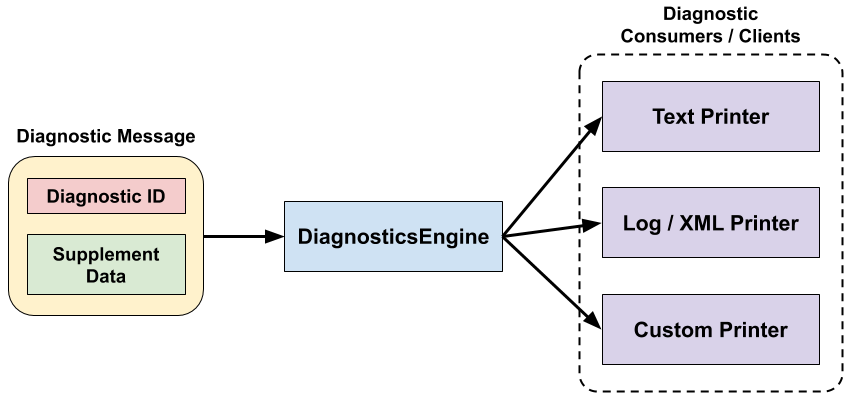
\includegraphics[width=0.9\textwidth]{content/2/chapter7/images/5.png}\\
图7.5 - Clang诊断框架的高层组织结构
\end{center}

\hspace*{\fill} \\ %插入空行
\noindent
\textbf{诊断信息}

从上图的左边开始,诊断消息——例如,使用未声明的标识符“x”——与具有自己诊断ID的消息模板相关联,“使用未声明的标识符消息”的消息模板如下所示:

\begin{tcblisting}{commandshell={}}
"use of undeclared identifier %0"
\end{tcblisting}

\texttt{\%0}是一个\textbf{占位符},稍后将由相应数据填充。本例中,它是具体的标识符名称(在前面的示例消息中是x)。\texttt{\%}后面的数字也表明了它将使用的数据。我们稍后将会详细讨论这种格式。

模板通过TableGen语法注册到诊断引擎。例如,这里讨论的消息模板就放在\texttt{clang/include/\\clang/Basic/DiagnosticSemaKinds.td}中:

\begin{lstlisting}[style=stylePython]
def err_undeclared_var_use : Error<"use of undeclared identifier %0">;
\end{lstlisting}

在前面的代码中,我们强调了两个部分。首先,这个消息模板的名称\texttt{err\_undeclare\_var\_use},稍后将用作唯一的诊断ID。第二,\texttt{Error}是一个带有错误消息的TableGen类,或者更正式地说,带有的是诊断级别错误。

总之,诊断消息由唯一的诊断ID(与消息模板及其诊断级别相关联)和数据组成,这些数据用于插入模板的占位符(如果有的话)。

\hspace*{\fill} \\ %插入空行
\noindent
\textbf{诊断用户}

诊断消息发送到诊断引擎(由\texttt{DiagnosticsEngine}类表示)之后,引擎将消息格式化为文本内容,并将它们发送给\textbf{诊断用户}(在代码库中也称为客户端)。

诊断用户(\texttt{DiagnosticConsumer}类的另一个实现)对从\texttt{DiagnosticsEngine}发送的文本消息进行处理后,通过不同的介质导出它们。例如,默认的\texttt{TextDiagnosticPrinter}将消息打印到命令行界面;另一方面,\texttt{LogDiagnosticPrinter}将传入消息打印到日志文件之前,会用简单的XML标记来进行装饰。理论上,可以创建一个自定义的\texttt{DiagnosticConsumer}来发送诊断消息到远程主机!

\hspace*{\fill} \\ %插入空行
\noindent
\textbf{报告诊断消息}

现在你已经了解了Clang的诊断框架是如何工作的,让我们了解一下如何发送(报告)诊断消息到诊断引擎:

\begin{enumerate}
\item 首先,需要检索对\texttt{DiagnosticEngine}的引用。这个引擎位于Clang编译管道的核心,所以可以从各种主组件中获取,比如:\texttt{ASTContext}和\texttt{SourceManager}。示例如下:

\begin{lstlisting}[style=styleJavaScript]
// `Ctx` has the type of `ASTContext&`
DiagnosticsEngine& Diag = Ctx.getDiagnostics();
\end{lstlisting}

\item 接下来,需要使用\texttt{DiagnosticsEngine::Report}函数,将诊断ID作为其参数之一,例如:报告\texttt{err\_undeclare \_var\_use}(在前面介绍过),就可以使用以下代码:

\begin{lstlisting}[style=styleJavaScript]
Diag.Report(diag::err_undeclared_var_use);
\end{lstlisting}

然而,\texttt{err\_undeclare\_var\_use}有一个占位符实参——即标识符名——通过\texttt{Report}函数和\texttt{<<}操作符来提供:

\begin{lstlisting}[style=styleJavaScript]
Diag.Report(diag::err_undeclared_var_use) << ident_name_str;
\end{lstlisting}

\item \texttt{err\_undeclare\_var\_use}只有一个占位符\texttt{\%0},所以会获取\texttt{<<}流中的第一个值。假设我们有一个诊断消息,\texttt{err\_invalid\_placement},使用下面的模板:

\begin{lstlisting}[style=styleJavaScript]
"you cannot put %1 into %0"
\end{lstlisting}

\item 可以使用下面的代码进行报告:
\begin{lstlisting}[style=styleJavaScript]
Diag.Report(diag::err_invalid_placement)
            << "boiling oil" << "water";
\end{lstlisting}

\item 除了简单的占位符之外,另一个有用的特性是\texttt{\%select}指令,例如:有一个诊断消息\texttt{warn\_exceed\_limit},模板如下:

\begin{lstlisting}[style=styleJavaScript]
"you exceed the daily %select{wifi|cellular network}0 limit"
\end{lstlisting}

\texttt{\%select}指令由大括号组成,其中不同的消息选项由\texttt{|}分隔。在大括号之外,前面代码中的一个数字(0)表示使用哪些数据来填充大括号内的选项。下面是一个例子:

\begin{lstlisting}[style=styleJavaScript]
Diag.Report(diag::warn_exceed_limit) << 1;
\end{lstlisting}

上面的代码将输出“\textbf{You exceed the daily cellular network limit}”。假设你使用0作为流操作符(<<)后面的参数:

\begin{lstlisting}[style=styleJavaScript]
Diag.Report(diag::warn_exceed_limit) << 0;
\end{lstlisting}

这将发出一个消息:超过了每天的wifi的流量限制(\textbf{you exceed the daily wifi limit})。

\item 假设使用另一个\texttt{Report}函数,它有一个\texttt{SourceLocation}参数:

\begin{lstlisting}[style=styleJavaScript]
// `SLoc` has the type of `SourceLocation`
Diag.Report(SLoc, diag::err_undeclared_var_use)
                  << ident_name_str;
\end{lstlisting}

输出消息将包含\texttt{SLoc}指向的部分源码:

\begin{tcblisting}{commandshell={}}
test.cc:2:10: error: use of undeclared identifier 'x'
  return x + 1;
          ^
\end{tcblisting}

\item 最后,尽管大多数诊断消息是通过Clang源代码树中的TableGen代码注册到\texttt{DiagnosticsEngine}的,但这并不意味着开发者可以在修改Clang源代码树的情况下创建新的诊断消息。让我们来看下\texttt{DiagnosticsEngine::getCustomDiagID(…)},这个API可以从一个消息模板和开发人员提供的诊断级别创建新的诊断ID:

\begin{lstlisting}[style=styleJavaScript]
auto MyDiagID = Diag.
getCustomDiagID(DiagnosticsEngine::Note,
"Today's weather is %0");
\end{lstlisting}

前面的代码创建的新诊断ID为\texttt{MyDiagID},它是在诊断级别上的消息模板,比如:\textbf{Today's weather is\%0}。可以像使用其他ID一样使用这个诊断ID:

\begin{lstlisting}[style=styleJavaScript]
Diag.Report(MyDiagID) << "cloudy";
\end{lstlisting}

\end{enumerate}

在本节中,了解了如何利用Clang的诊断框架来打印消息,就像普通编译器消息一样。

接下来,我们将结合本章学到的所有技能来创建一个自定义的AST插件。

\subsubsubsection{7.3.3\hspace{0.2cm}创建AST插件}

本章的前几节中,我们探索了Clang的AST,并了解了如何在内存API中使用。本节中,我们来了解如何编写一个插件,以一种简单的方式将自定义的AST处理逻辑插入到Clang的编译管道中。

在第5章,我们了解了使用Clang (AST)插件的优势:即使使用一个预构建的Clang可执行文件,也可以进行开发使用,插件很容易编写,可以与现有的工具链和构建系统有很好的集成等。在第6章中,我们开发了一个用于预处理器中自定义编译处理的插件。本章中,我们还将编写一个插件,但这个插件为自定义AST处理而设计。这两个插件的代码框架也有很大的不同。

我们在项目概述一节中介绍了本节将使用的示例项目。如果输入代码中的某些\texttt{if-else}语句可以转换成三元运算符,这个插件会提示用户警告消息。此外,它还显示了关于构建三元操作符的候选表达式的提示。

下面是构建插件的详细步骤:

\begin{enumerate}
\item 与我们在第6章中看到的pragma插件类似,在Clang中创建一个插件基本上就像实现一个类。在开发AST插件时,将使用\texttt{PluginASTAction}类。

\texttt{PluginASTAction}是\texttt{ASTFrontendAction}的子类——专门用于处理AST的\texttt{FrontendAction}(如果你不熟悉\texttt{FrontendAction},可以回顾一下第5章的内容)。因此,我们需要实现\texttt{CreateASTConsumer}成员函数:

\begin{lstlisting}[style=styleCXX]
struct TernaryConverterAction : public PluginASTAction {
	std::unique_ptr<ASTConsumer>
	CreateASTConsumer(CompilerInstance &CI,
                      StringRef InFile) override;
};
\end{lstlisting}

我们将在稍后填充这个函数。

\item 除了\texttt{CreateASTConsumer}外,还可以重写另外两个成员函数来更改一些功能:\texttt{getActionType}和\texttt{ParseArgs}。前者告诉Clang如何执行这个插件,返回一个枚举值如下所示:

\begin{enumerate}[label=\alph*.]
\item \texttt{Cmdline}: 如果用户提供\texttt{-plugin <plugin name>}(前端的)命令行标志,插件将在主操作之后执行。

\item \texttt{ReplaceAction}: 这取代了Clang将要执行的原始动作,例如:Clang将输入代码编译到一个目标文件(\texttt{-c}标志)时,则执行插件的动作(而不是在插件加载时执行)。

\item \texttt{AddBefore/AfterMainAction}: 原来的Clang动作仍然会执行,并且插件动作会添加到它的前面或后面执行。
\end{enumerate}

这里,我们将使用\texttt{Cmdline}操作类型:

\begin{lstlisting}[style=styleCXX]
struct TernaryConverterAction : public PluginASTAction {
	…
	ActionType getActionType() override { return Cmdline; }
};
\end{lstlisting}

另一方面,\texttt{ParseArgs}成员函数处理(前端的)特定于这个插件的命令行选项。换句话说,可以为插件创建自定义命令行标志。我们的例子中,将创建两个标志:\texttt{-no-detect-return}和\texttt{-no-detect-assignment}。这允许我们决定是否希望检测返回语句或赋值语句的(潜在)三元转换:

\begin{lstlisting}[style=styleCXX]
struct TernaryConverterAction : public PluginASTAction {
	…
	bool NoAssignment = false,
	NoReturn = false;
	bool ParseArgs(const CompilerInstance &CI,
	const std::vector<std::string> &Args) override {
		for (const auto &Arg : Args) {
			if (Arg == "-no-detect-assignment") NoAssignment =
			true;
			if (Arg == "-no-detect-return") NoReturn = true;
		}
	    return true;
    }
};
\end{lstlisting}

如上面的代码所示,我们创建了两个布尔标记,\texttt{NoReturn}和\texttt{NoAssignment},来存储命令行选项的值。\texttt{ParseArgs}的返回值非常重要,\texttt{ParseArgs}实际上是在返回插件\textit{是否应该继续执行},而不是返回\textit{是否解析了任何自定义标志}。因此,在大多数情况下,总是返回true。

\item 现在,我们将讨论\texttt{CreateASTConsumer}的内容。这个函数将返回一个\texttt{ASTConsumer}对象,它是自定义的逻辑主体。然而,我们不打算直接实现\texttt{ASTConsumer}。相反,我们\texttt{ASTConsumer}对象是由\textit{ASTMatcher}生成的(已经在本章的前面内容中介绍过)。

构建\texttt{MatchFinder}实例需要两个东西——\texttt{ASTMatcher}中的主要模式匹配驱动(用ASTMatcher自己的DSL编写的模式)和一个\texttt{MatchCallback}实现。我们将模式和匹配器回调分为两类:基于\texttt{return}语句检测可能的三元操作符的模式,以及\textit{基于赋值语句检测的模式}。

以下是\texttt{CreateASTConsumer}的框架:

\begin{lstlisting}[style=styleCXX]
using namespace ast_matchers;
struct TernaryConverterAction : public PluginASTAction {
	…
private:
	std::unique_ptr<MatchFinder> ASTFinder;
	std::unique_ptr<MatchFinder::MatchCallback>
	  ReturnMatchCB, AssignMatchCB;
};

std::unique_ptr<ASTConsumer>
TernaryConverterAction::CreateASTConsumer
(CompilerInstance &CI, StringRef InFile) {
	ASTFinder = std::make_unique<MatchFinder>();
	// Return matcher
	if (!NoReturn) {
		ReturnMatchCB = /*TODO: Build MatcherCallback
		instance*/
		ASTFinder->addMatcher(traverse
		  (TK_IgnoreUnlessSpelledInSource,
		    /*TODO: Patterns in DSL*/), ReturnMatchCB.get());
	}
	// Assignment matcher
	if (!NoAssignment) {
		AssignMatchCB = /*TODO: Build MatcherCallback
		  instance*/
		ASTFinder->addMatcher(traverse
		  (TK_IgnoreUnlessSpelledInSource,
		    /*TODO: Patterns in DSL*/), AssignMatchCB.get());
	}
	return std::move(ASTFinder->newASTConsumer());
}
\end{lstlisting}

前面的代码创建了三个\texttt{unique\_ptr}类型成员变量:一个用于存储\texttt{MatchFinder},两个存储\texttt{MatchCallback}的用于基于返回和基于分配的模式。

\begin{tcolorbox}[colback=blue!5!white,colframe=blue!75!black, fonttitle=\bfseries,title=为啥使用unique\_ptr?]	\hspace*{0.7cm}使用\texttt{unique\_ptr}来存储这三个对象——或者持久化存储这些对象——背后的原理是因为,要在\texttt{CreateASTConsumer (ASTFinder->newASTConsumer())}末尾创建的\texttt{ASTConsumer}实例保留了对这三个对象的引用。因此,我们需要一种方法来保持它们在前端的生命周期内的存活性。
\end{tcolorbox}

除此之外,通过使用\texttt{MatchFinder::addMatcher}、\texttt{traverse}函数和\texttt{MatchCallback}实例,在\texttt{MatchFinder}中注册了遍历模式。如果不熟悉这些API,请会看关于\texttt{ASTMatcher}的部分章节。

现在,我们只需要组合匹配模式,并实现一些回调,以便在存在匹配时打印出警告消息——如前面代码中建议的\texttt{TODO}注释所示。

\item 先来处理模式。我们正在寻找的模式——基于返回和基于赋值的模式——在最外层的布局中有一个函数(\texttt{FunctionDecl}表示整个函数,\texttt{CompoundStmt}表示函数体)包围的\texttt{if-else}语句(\texttt{IfStmt})。两者内部,\texttt{IfStmt}的真分支和假分支中,只能存在一条语句。这个结构可以这样描述:

\begin{tcolorbox}[colback=white,colframe=black]
\tt
\zihao{-5}
FunctionDecl \\
\hspace*{0.3cm}|\_CompoundStmt \\
\hspace*{0.6cm}|\_(Other AST nodes we don't care) \\
\hspace*{0.6cm}|\_IfStmt \\
\hspace*{0.9cm}|\_(true branch: contain only one return/assign statement) \\
\hspace*{0.9cm}|\_(false branch: contain only one return/assign statement)
\end{tcolorbox}

为了将这个概念转换成ASTMatcher的DSL,下面是基于返回值和基于分配的模式之间共享的DSL代码:

\begin{lstlisting}[style=styleCXX]
functionDecl(
compoundStmt(hasAnySubstatement
		IfStmt(
			hasThen(/*TODO: Sub-pattern*/)
			hasElse(/*TODO: Sub-pattern*/)
		)
	)
);
\end{lstlisting}

要记住,当处理\texttt{CompoundStmt}时,应该使用限定指令,比如:让\texttt{hasAnySubstatement}来匹配它的主体语句。

我们将使用前面的\texttt{TODO}注释来定制这些基于返回值或基于分配的情况。来使用子模式变量来替换那些\texttt{TODO}注释,并把前面的代码放到另一个函数中:

\begin{lstlisting}[style=styleCXX]
StatementMatcher
buildIfStmtMatcher(StatementMatcher truePattern,
				   StatementMatcher falsePattern) {
	return functionDecl(
	  compoundStmt(hasAnySubstatement
  	    IfStmt(
		  hasThen(truePattern)
		  hasElse(falsePattern))));
}
\end{lstlisting}

\item 对于基于返回值的模式,相对于上一步中提到的两个\texttt{if-else}分支的子模式是稍微复杂一些。这里,我们也使用了一个单独的函数来创建这个模式:

\begin{lstlisting}[style=styleCXX]
StatementMatcher buildReturnMatcher() {
	return compoundStmt(statementCountIs(1),
						hasAnySubstatement(
						returnStmt(
						hasReturnValue(expr()))));
}
\end{lstlisting}

如上面的代码所示,我们使用\texttt{statementCountIs}指令将代码块与只有一条语句匹配。此外,还通过\texttt{hasReturnValue(…)}指定了不为空的返回值。\texttt{hasReturnValue}参数是必要的,因为后者至少接受一个参数,但由于我们不关心什么类型的节点,所以使用\texttt{expr()}作为某种通配符模式。

对于基于赋值的模式,事情变得有点复杂:我们不只是想在两个分支中匹配单个赋值语句(由\texttt{BinaryOperator}类建模)——这些赋值的LHS需要是指向同一个\texttt{Decl}实例的\texttt{DeclRefExpr}表达式。不幸的是,我们不能使用ASTMatch的DSL来表达这些谓词。然而,可以将一些检查推到\texttt{MatchCallback}中,并且只使用DSL指令来检查我们想要的模式\textit{形状}:

\begin{lstlisting}[style=styleCXX]
StatementMatcher buildAssignmentMatcher() {
	return compoundStmt(statementCountIs(1),
						hasAnySubstatement(
						binaryOperator(
						hasOperatorName("="),
						hasLHS(declRefExpr())
						)));
}
\end{lstlisting}

\item 现在我们已经完成了模式的框架,是时候来实现\texttt{MatchCallback}了。在\texttt{MatchCallback::run}中我们会做两件事。首先,对于基于分配的模式,检查那些匹配的分配候选LHS的\texttt{DeclRefExpr}是否指向相同的\texttt{Decl}。其次,打印出帮助用户将\texttt{if-else}分支重写为三元运算符的消息。换句话说,我们需要一些匹配的AST节点的位置信息。

让我们使用\textit{AST节点绑定技术}来解决第一个任务。计划是绑定候选赋值的LHS \texttt{DeclRefExpr}节点,这样就可以从\texttt{MatchCallback::run}中对它们进行检索,并对它们的\texttt{Decl}节点执行进一步的检查。我们来对\texttt{buildAssignmentMatch}进行修改:

\begin{lstlisting}[style=styleCXX]
StatementMatcher buildAssignmentMatcher() {
	return compoundStmt(statementCountIs(1),
						hasAnySubstatement(
						binaryOperator(
						hasOperatorName("="),
						hasLHS(declRefExpr().
						bind("dest")))));
}
\end{lstlisting}

尽管前面的代码看起来很简单,但是在这个绑定方案中有一个问题:在两个分支中,\texttt{DeclRefExpr}的绑定使用了相同的名称,这意味着后面出现的AST节点将覆盖之前绑定的节点。因此,我们不会像之前计划的那样从两个分支获得\texttt{DeclRefExpr}节点。

因此,这里为\texttt{DeclRefExpr}使用一个不同的标签来匹配两个分支:\texttt{dest.true}表示真分支,\texttt{dest.false}表示假分支。让我们调整前面的代码来反映这个策略:

\begin{lstlisting}[style=styleCXX]
StatementMatcher buildAssignmentMatcher(StringRef Suffix)
{
	auto DestTag = ("dest" + Suffix).str();
	return compoundStmt(statementCountIs(1),
						hasAnySubstatement(
						binaryOperator(
						hasOperatorName("="),
						hasLHS(declRefExpr().
						bind(DestTag)))));
}
\end{lstlisting}

当调用\texttt{buildAssignmentMatcher}时,我们将为不同的分支传递不同的后缀——或者是\texttt{.true}或者\texttt{.false}。

最后,必须在\texttt{MatchCallback::run}中检索绑定的节点。这里,我们为基于返回和基于分配的场景创建了不同的\texttt{MatchCallback}子类——分别是\texttt{MatchReturnCallback}和\texttt{MatchAssi\\gnmentCallback}。下面是\texttt{MatchAssignmentCallback::run}中的部分代码:

\begin{lstlisting}[style=styleCXX]
void
MatchAssignmentCallback::run(const MatchResult &Result)
override {
	const auto& Nodes = Result.Nodes;
	// Check if destination of both assignments are the
	// same
	const auto *DestTrue =
			Nodes.getNodeAs<DeclRefExpr>("dest.true"),
			*DestFalse =
			Nodes.getNodeAs<DeclRefExpr>("dest.false");
	if (DestTrue->getDecl() == DestFalse->getDecl()) {
		// Can be converted into ternary operator!
	}
}
\end{lstlisting}

我们将在下一步解决第二个任务——打印有用的信息给用户。

\item 要打印有用的信息——包括代码的哪一部分可以转换成三元运算符,以及如何构建三元运算符——需要在获取其源位置信息之前,从匹配的模式中检索一些AST节点。为此,我们将使用一些节点绑定技巧。这一次,我们将修改所有的模式构建功能,也就是\texttt{buildIfStmtMatcher}、\texttt{buildReturnMatcher}和\texttt{builassignmentmatcher}:

\begin{lstlisting}[style=styleCXX]
StatementMatcher
buildIfStmtMatcher(StatementMatcher truePattern,
				   StatementMatcher falsePattern) {
	return functionDecl(
		compoundStmt(hasAnySubstatement
			IfStmt(
				hasThen(truePattern)
				hasElse(falsePattern)).bind("if_stmt")
		));
}
\end{lstlisting}

这里,对匹配的\texttt{IfStmt}进行了绑定,因为我们想告诉用户,哪些地方可以转换为三元操作符:

\begin{lstlisting}[style=styleCXX]
StatementMatcher buildReturnMatcher(StringRef Suffix) {
	auto Tag = ("return" + Suffix).str();
	return compoundStmt(statementCountIs(1),
						hasAnySubstatement(
						  returnStmt(hasReturnValue(
						    expr().bind(Tag)
						  ))));
}
StatementMatcher buildAssignmentMatcher(StringRef Suffix)
{
	auto DestTag = ("dest" + Suffix).str();
	auto ValTag = ("val" + Suffix).str();
	return compoundStmt(statementCountIs(1),
						hasAnySubstatement(
						binaryOperator(
						hasOperatorName("="),
						hasLHS(declRefExpr().
						bind(DestTag)),
						hasRHS(expr().bind(ValTag))
						)));
}
\end{lstlisting}

在这里使用的节点绑定技巧与前面的代码中使用的相同。在此之后,我们可以从\texttt{MatchCall\\back::run}中检索那些绑定的节点,并使用这些节点的\texttt{SourceLocation}信息进行打印。

我们将在这里使用Clang的诊断框架来打印这些消息。由于预期的消息格式在Clang的代码库中并不存在,我们将通过\texttt{DiagnosticsEngine::getCustomDiagID(…)}创建自己的诊断ID。下面是我们在\texttt{MatchAssignmentCallback::run}中做的事情(因为\texttt{MatchReturnCallback}是类似的,所以这里只演示\texttt{MatchAssignmentCallback}):

\begin{lstlisting}[style=styleCXX]
void
MatchAssignmentCallback::run(const MatchResult &Result)
override {
	…
	auto& Diag = Result.Context->getDiagnostics();
	auto DiagWarnMain = Diag.getCustomDiagID(
	  DiagnosticsEngine::Warning,
	  "this if statement can be converted to ternary
	    operator:");
	    
	auto DiagNoteTrueExpr = Diag.getCustomDiagID(
	  DiagnosticsEngine::Note,
	  "with true expression being this:");
	  
	auto DiagNoteFalseExpr = Diag.getCustomDiagID(
	  DiagnosticsEngine::Note,
	  "with false expression being this:");
	…
}
\end{lstlisting}

结合绑定节点检索,下面是如何打印消息:

\begin{lstlisting}[style=styleCXX]
void
MatchAssignmentCallback::run(const MatchResult &Result)
override {
	…
	if (DestTrue && DestFalse) {
		if (DestTrue->getDecl() == DestFalse->getDecl()) {
			// Can be converted to ternary!
			const auto* If = Nodes.getNodeAs<IfStmt>
			("if_stmt");
			Diag.Report(If->getBeginLoc(), DiagWarnMain);
			
			const auto* TrueValExpr =
			            Nodes.getNodeAs<Expr>("val.true");
			const auto* FalseValExpr =
			            Nodes.getNodeAs<Expr>("val.false");
			Diag.Report(TrueValExpr->getBeginLoc(),
			            DiagNoteTrueExpr);
			Diag.Report(FalseValExpr->getBeginLoc(),
			            DiagNoteFalseExpr);
		}
	}
}
\end{lstlisting}

\item 最后,返回\texttt{CreateASTConsumer}。下面展示了,是所有内容是如何拼凑起来的:

\begin{lstlisting}[style=styleCXX]
std::unique_ptr<ASTConsumer>
TernaryConverterAction::CreateASTConsumer(
CompilerInstance &CI, StringRef InFile) {
	…
	// Return matcher
	if (!NoReturn) {
	ReturnMatchCB = std::make_unique<MatchReturnCallback>();
      ASTFinder->addMatcher(
	    traverse(TK_IgnoreUnlessSpelledInSource,
	             buildIfStmtMatcher(
	             buildReturnMatcher(".true"),
	             buildReturnMatcher(".false"))),
	    ReturnMatchCB.get()
	  );
 	}

	// Assignment matcher
	if (!NoAssignment) {
	AssignMatchCB = std::make_
	  unique<MatchAssignmentCallback>();
	ASTFinder->addMatcher(
	    traverse(TK_IgnoreUnlessSpelledInSource,
	             buildIfStmtMatcher(
	             buildAssignmentMatcher(".true"),
	             buildAssignmentMatcher(".false"))),
	    AssignMatchCB.get()
	  );
	}

	return std::move(ASTFinder->newASTConsumer());
}
\end{lstlisting}

这就是我们要做的所有事情!

\item 最后,运行插件的命令:

\begin{tcblisting}{commandshell={}}
$ clang -fsyntax-only -fplugin=/path/to/TernaryConverter.
so -Xclang -plugin -Xclang ternary-converter \
  test.c
\end{tcblisting}

将得到一个类似于在\textbf{项目概述}中看到的输出。

要在这个项目中使用插件特定的标志,比如\texttt{-no-detect-return}和\texttt{-no-detectassignment},请在这里显式添加命令行选项:

\begin{tcblisting}{commandshell={}}
$ clang -fsyntax-only -fplugin=/path/to/TernaryConverter.
so -Xclang -plugin -Xclang ternary-converter \
   -Xclang -plugin-arg-ternary-converter \
   -Xclang -no-detect-return \
    test.c
\end{tcblisting}

更具体地说,要以\texttt{-plugin-arg-<plugin name>}格式添加第一个高亮显示的参数。

\end{enumerate}

本节中,了解了如何编写AST插件,该插件在有\texttt{if-else}语句时向用户发送消息,表明该语句可以转换为三元操作符。可以利用本章所介绍的所有技术来做其他的事情,例如:Clang AST的内存表示、ASTMatcher和诊断框架。





















